
\subsection{Trajectory clustering distinguishes distinct lineages in HSC differentiation}

We sought to test our trajectory featurization approach in a differentiation model with clearly defined endpoints, in order to compare clustering on trajectory features to ground-truth cell types. We chose a multi-omic time course dataset of human hematopoietic stem cells (HSCs), which cross sections their development at days 2, 3, 4, and 7 after induction of differentiation \citep{danielburkhardtOpenProblemsMultimodal2022}.

\begin{figure}[ht]
    \centering
    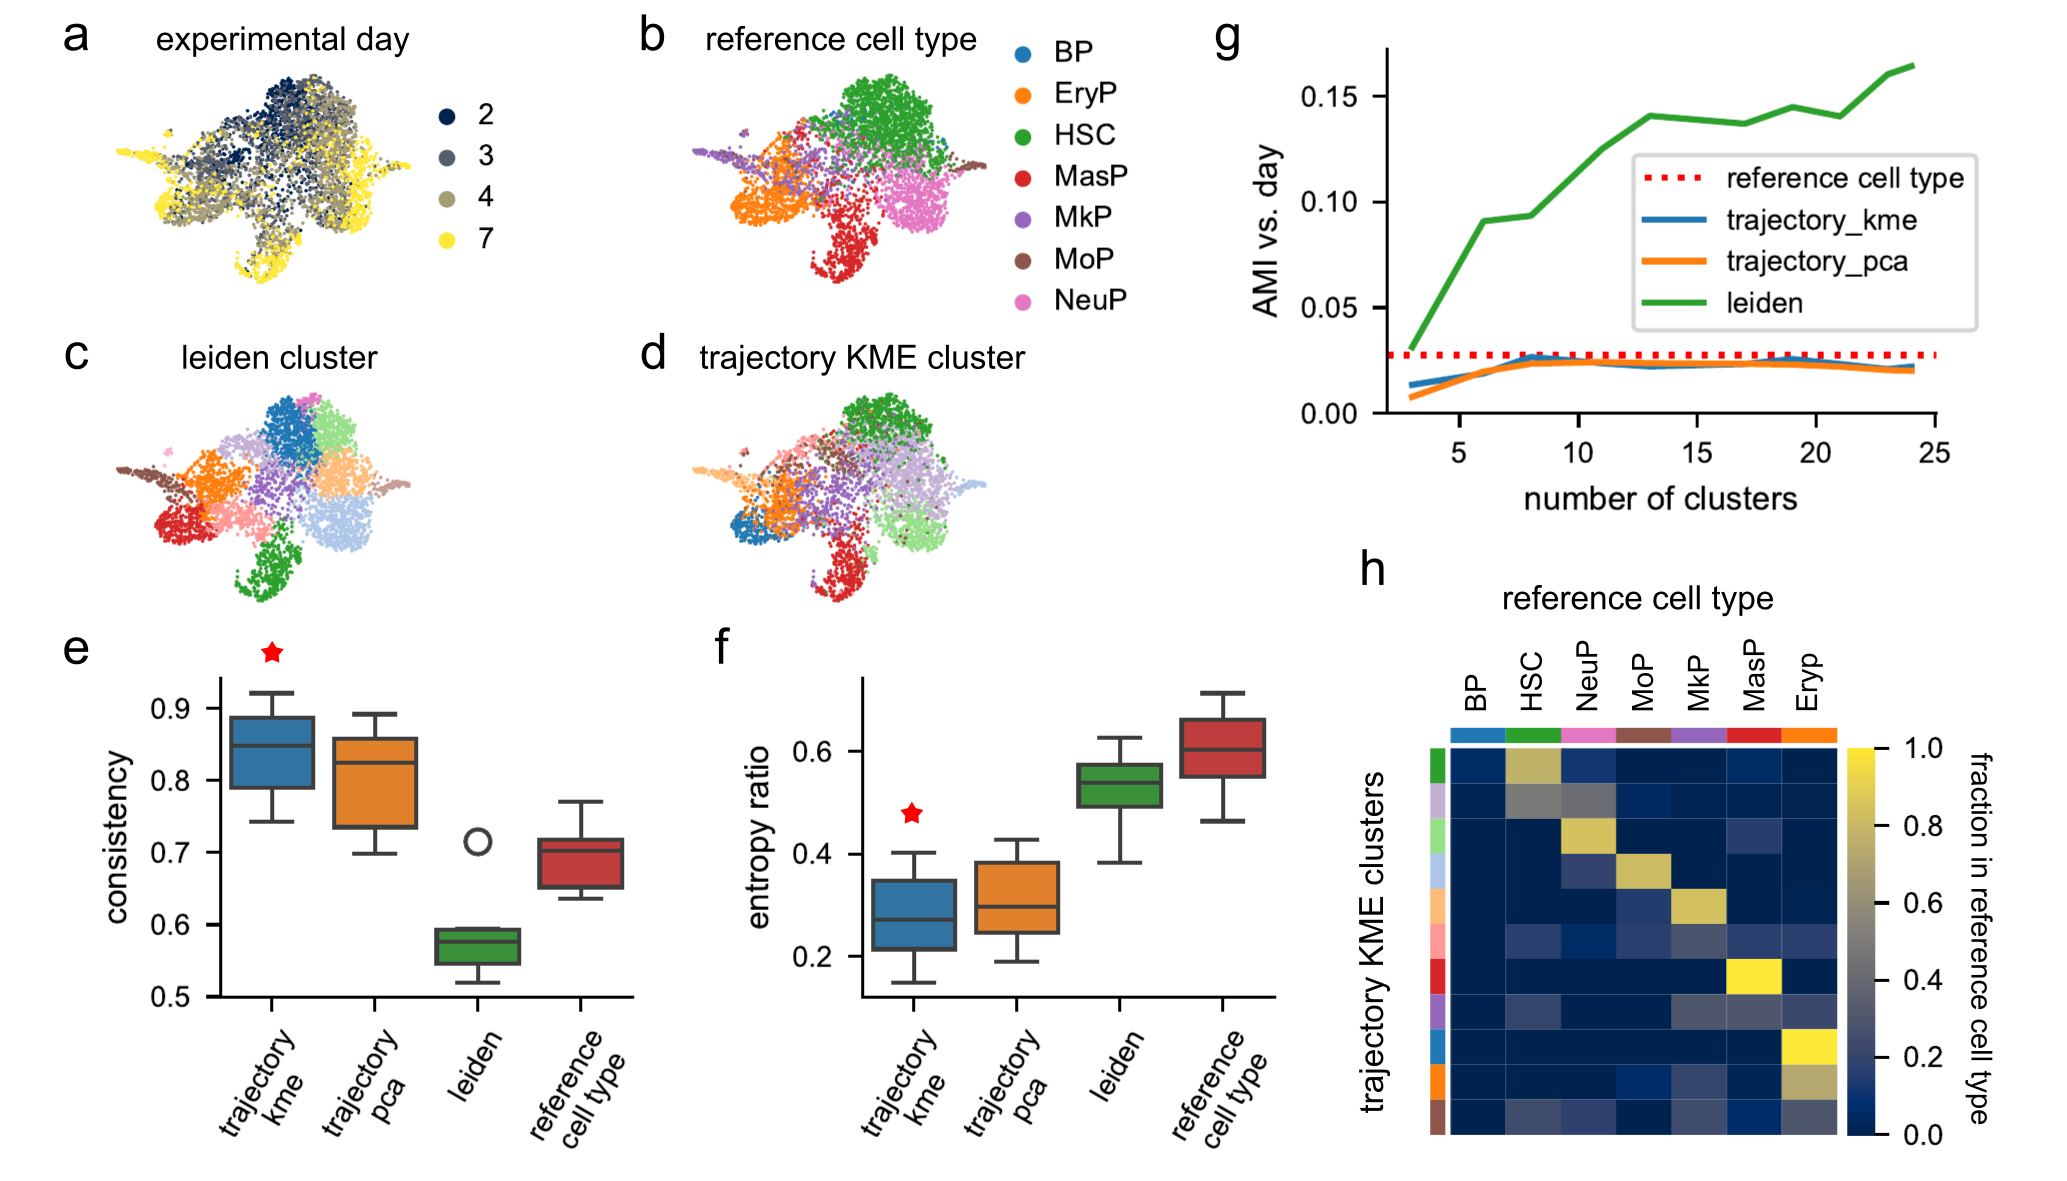
\includegraphics[width=\linewidth]{ch2/figs/Results_moscot_hsc_20250212.png}
    \caption[Clustering on trajectory features accurately partitions cell types in HSCs and streamlines cluster flows.]{
    Clustering on trajectory features accurately partitions cell types in HSCs and streamlines cluster flows. 
    (a-d) UMAP dimensionality reductions showing (a) experimental day, (b) reference cell type labels, (c) Leiden clusters, and (d) k-means clusters fit on trajectory KME features.
    (e-f) Boxplots evaluating how well clusters represent the underlying trajectory model, using (e) flow consistency score and (f) entropy ratio score. The best performing clusters for each metric are annotated using a red star.
    (g) Line plot showing adjusted mutual information (AMI) between clusters and experimental day, versus the input number of clusters for different clustering methods. The AMI between the reference cell types and experimental day is displayed by a dotted red line.
    (h) Heatmap colored by the fraction of each trajectory cluster (rows) overlapping with a given reference cell type (columns) at day 7.
    }
    \label{fig:hsc}
    \label{fig:hsc-a}
    \label{fig:hsc-b}
    \label{fig:hsc-c}
    \label{fig:hsc-d}
    \label{fig:hsc-e}
    \label{fig:hsc-f}
    \label{fig:hsc-g}
    \label{fig:hsc-h}
\end{figure}

Data were downloaded through the moscot Python package \citep{kleinMappingCellsTime2023a}, and included labeled cell types, as well as uniform manifold approximation and projection (UMAP) dimensionality reductions for both RNA and ATAC modalities. We constructed a shared embedding representation from both data modalities and fit the trajectory model on these shared coordinates using moscot. We then used the fitted model to construct single-cell trajectory feature vectors, using either an RBF feature map (trajectory KME) or PCA decomposition (trajectory PCA) as the featurization function.


We fit k-means clusters on both sets of trajectory features, and compared these against the reference cell types as well as Leiden clusters fit using only gene expression information. Uniform manifold approximation and projection in the gene expression space (UMAP) showed that most cells belong to the HSC reference cell type at day 2, and proceed to differentiate into various lineages from days 3-7 (Fig~\ref{fig:hsc-a}a-b). The Leiden clusters appear to split many of the reference cell types into groups, especially the undifferentiated HSC cluster (Fig~\ref{fig:hsc-c}c). The trajectory KME clusters similarly partition the reference cell types (Fig~\ref{fig:hsc-d}d), however they exhibit less sharp boundaries between clusters than the Leiden clusters. At the termini of the  differentiation trajectory, both Leiden and trajectory KME clusters appear to align strongly with the reference cell types. Indeed, Fig~\ref{fig:hsc-h}h shows that most of the trajectory KME clusters at day 7 correspond to a single reference cell type.

We next evaluated the performance of the clustering methods in capturing trajectory information using the flow consistency \eqref{eq:flow_consistency} and flow entropy \eqref{eq:flow_entropy} scores. We see that both trajectory clusters exhibit high consistency and low entropy compared to the Leiden clusters and reference cell types (Fig~\ref{fig:hsc-e}e-f), suggesting that both featurization strategies are successfully encoding information about cellular trajectories. The trajectory KME clusters slightly outperform the trajectory PCA clusters for both metrics, which hints at their greater ability to represent higher-order distributional information. Nonetheless, the trajectory PCA clusters perform quite well,  perhaps due to the simplicity of the bifurcations in this dataset. In contrast, the reference clusters show the highest flow entropy of any clustering (Fig~\ref{fig:hsc-f}f), likely driven by the ability of the multipotent HSC cell type to give rise to different populations.

Interestingly, the Leiden clusters showed exceptionally low flow consistency (Fig~\ref{fig:hsc-e}e). We hypothesized that this could be because the Leiden clusters are separating by experimental day more than the other clusters. This would cause the trajectories to switch clusters more often between time points, resulting in a lower consistency score. We tested this by measuring the adjusted mutual information (AMI) between each set of clusters and experimental day. We see that the Leiden clusters have higher AMI with experimental day than any of the other clusters (Fig~\ref{fig:hsc-g}g). Furthermore, increasing the number of clusters caused the Leiden clusters to correlate more strongly with time point, but did not affect the trajectory clusters. Trajectory featurization may therefore be a useful strategy for removing confounding effects due to time during single-cell phenotyping. 

\subsection{Characterizing perturbation responses using trajectory divergence}

\begin{figure}[ht]
    \centering
    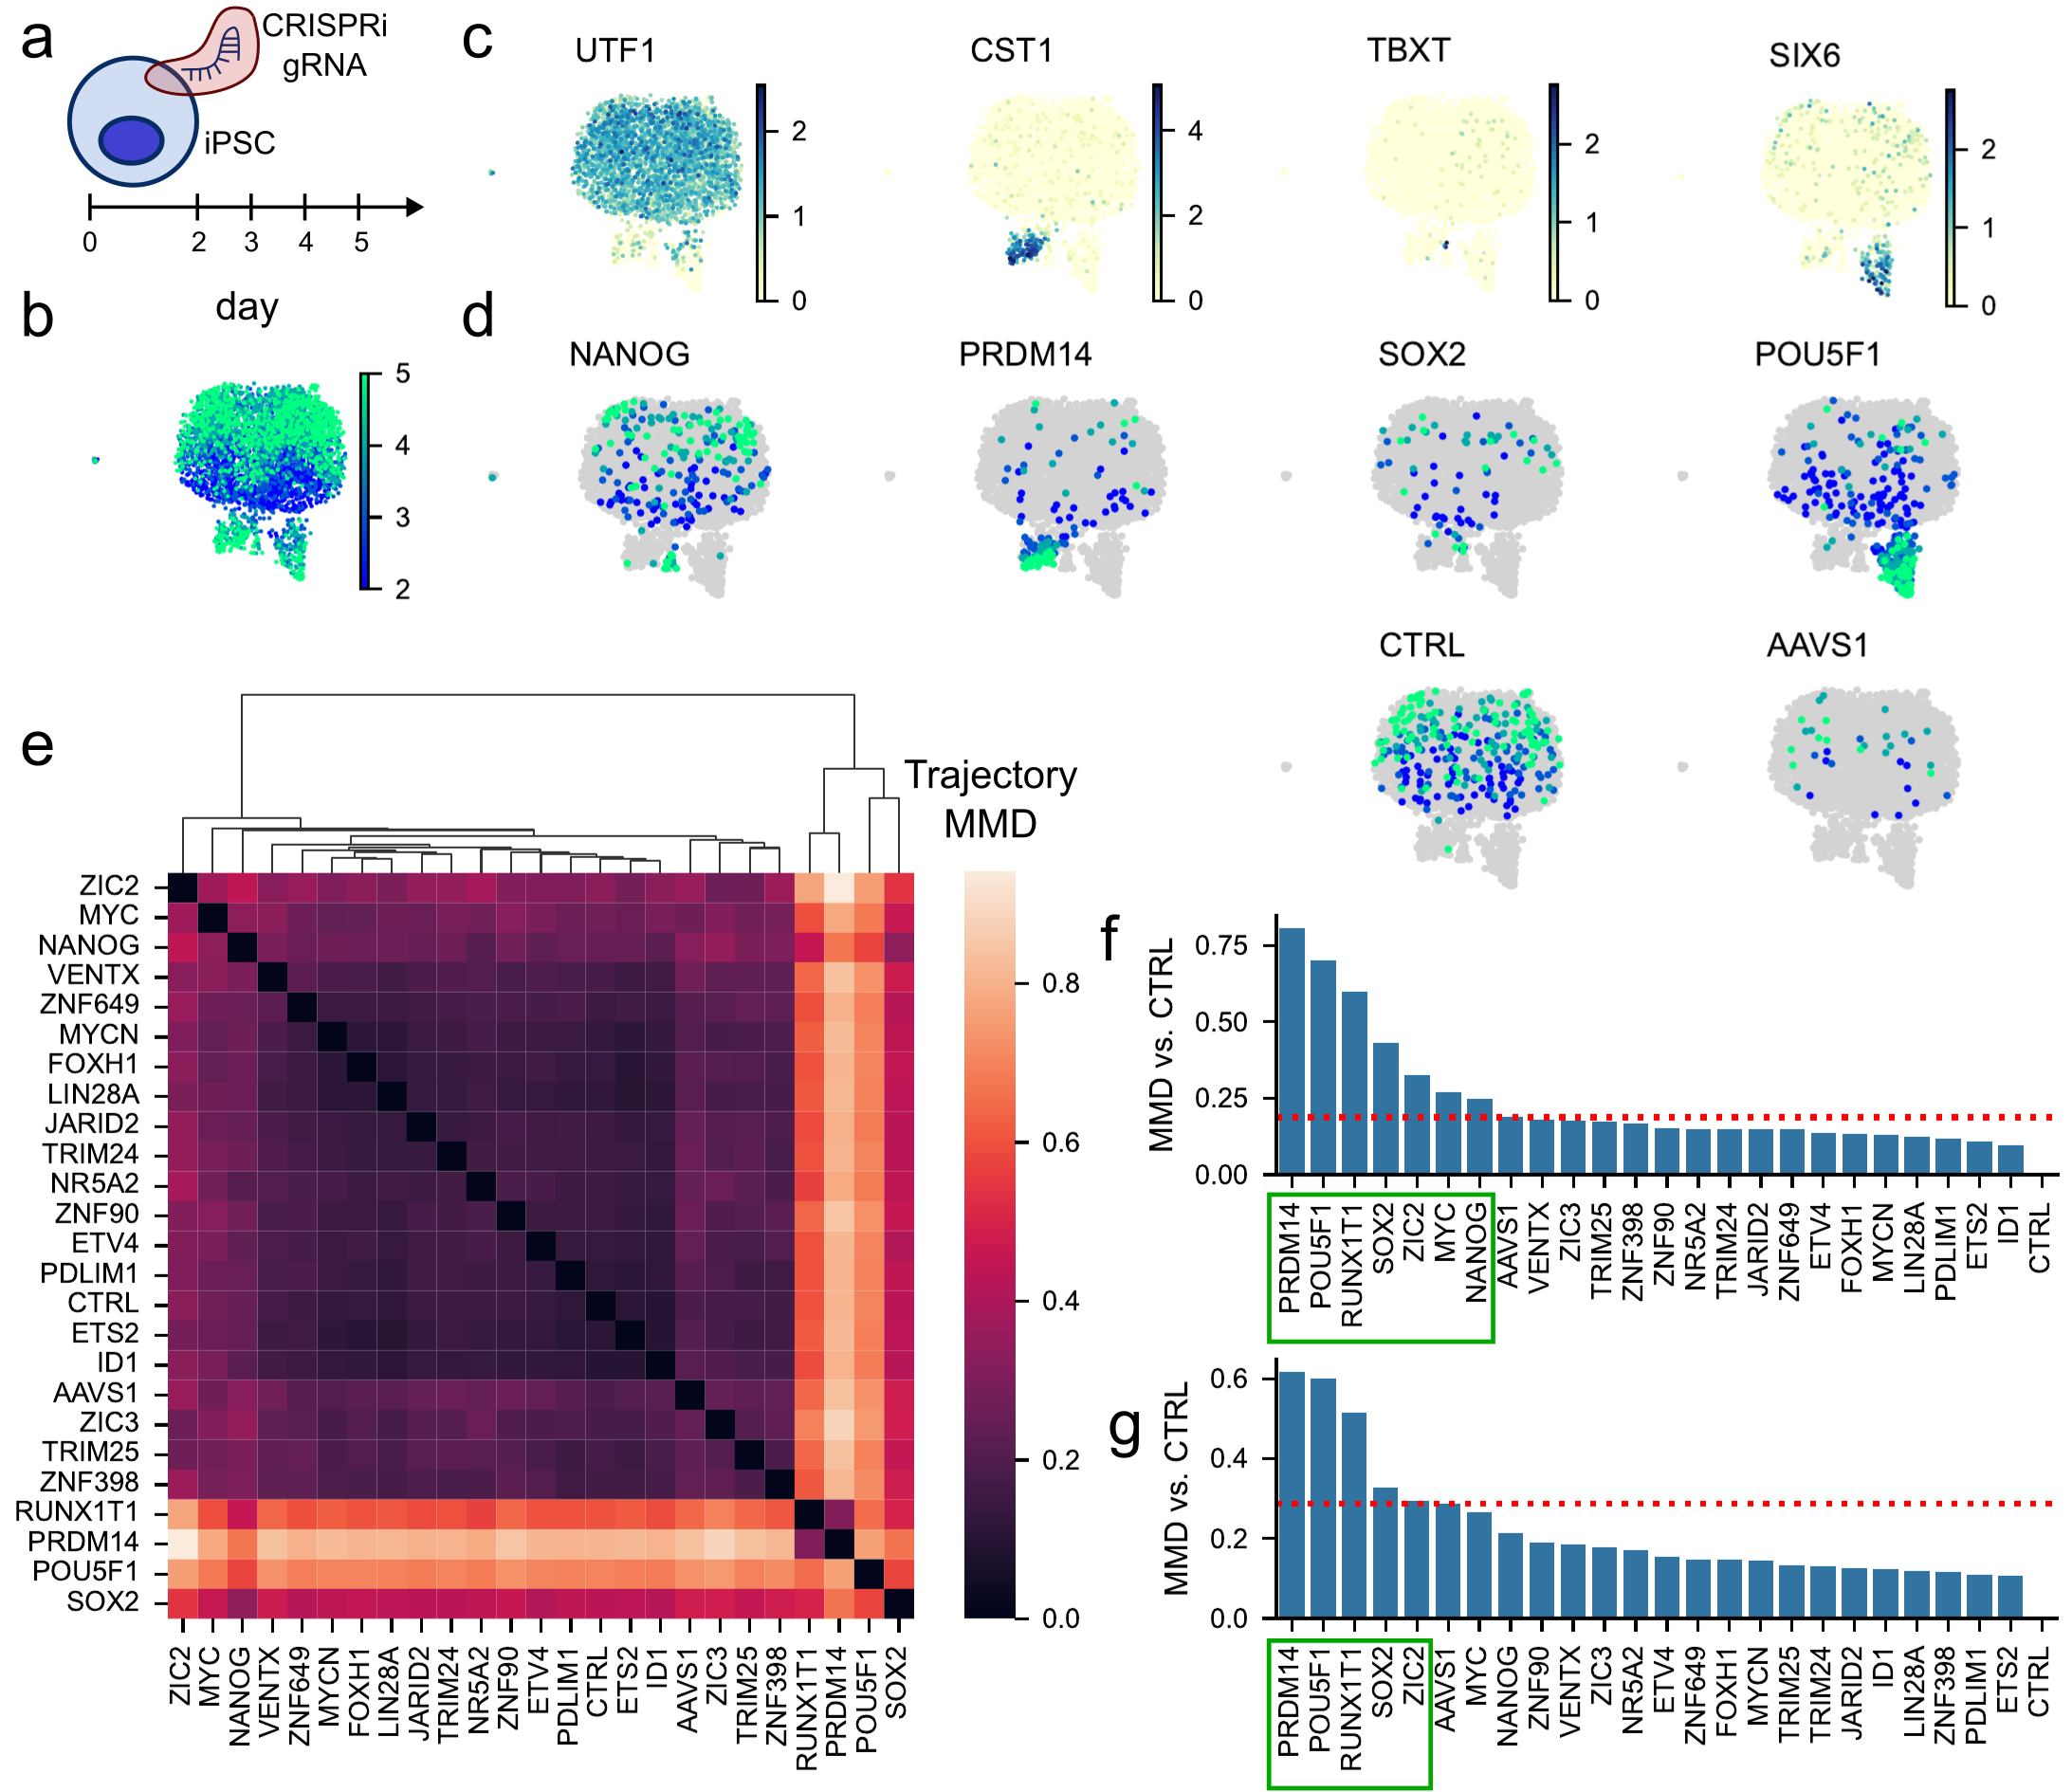
\includegraphics[width=\textwidth]{ch2/figs/Results_Ishikawa_iPSC_perturbation.png}
    \caption[Comparison of iPSC responses to CRISPRi perturbation using trajectory divergence demonstrates enhanced ability to identify significant responses compared to using a single time point.]{
    Comparison of iPSC responses to CRISPRi perturbation using trajectory divergence demonstrates enhanced ability to identify significant responses compared to using a single time point.
    (a) The dataset follows differentiation iPSCs in response to a panel of 50 CRISPRi guide RNAs targeting 25 transcription factors at days 2-5 following induction.
    (b) UMAP displaying the days at which each cell was collected.
    (c) UMAPs displaying normalized gene expression of pluripotent (\textit{UTF1}), definitive endoderm (\textit{CST1}), axial mesoderm (\textit{TBXT}), and neural (\textit{SIX6}) lineage markers.
    (d) UMAPs showing distributions of cells expressing a single gRNA, colored by sampling time. Cells without the gRNA are grayed-out.
    (e) Heatmap of MMD between trajectory kernel mean embeddings for each pair of perturbations.
    (f) Trajectory MMD between each perturbation and the control condition. Perturbations with MMDs greater those targeting the non-coding AAVS1 locus (red dotted line) are shown in the green box.
    (g) MMD between each perturbation and the control condition, computed using cells and features from day 5 only. Perturbations with MMDs greater those targeting the non-coding AAVS1 locus (red dotted line) are shown in the green box.
    }
    \label{fig:ipsc}
    \label{fig:ipsc-a}
    \label{fig:ipsc-b}
    \label{fig:ipsc-c}
    \label{fig:ipsc-d}
    \label{fig:ipsc-e}
    \label{fig:ipsc-f}
    \label{fig:ipsc-g}
\end{figure}

One of the advantages of using trajectory mean embeddings during data analysis is that they naturally induce the maximum mean discrepancy (MMD) metric on probability distributions. Here, we show how this can be used to analyze combined perturbation and time course single-cell data, to recover perturbations with substantial time-dependent effects on cell state. We performed reanalysis on the dataset from \cite{ishikawaRENGEInfersGene2023}, which features differentiation induced pluripotent stem cells (iPSCs) under the influence of CRISPRi guide RNAs targeting 25 transcription factors (TFs). iPSCs were profiled using scRNA-seq on each day from days 2-5 following induction (Fig~\ref{fig:ipsc-a}a). Thus, this dataset presents a unique opportunity to show how using trajectory analysis can increase power to detect perturbation responses.

The gRNA expression from each cell was log1p-transformed, and then binarized using Otsu thresholding. We selected cells expressing exactly one gRNA, and then preprocessed the RNA data using a standard analysis pipeline. UMAP dimensionality reduction showed that the cells start in an intermediate state and branch outwards over time (Fig~\ref{fig:ipsc-b}b). Each major branch expressed some lineage marker genes, with the largest branch being defined by the pluripotency marker \textit{UTF1}, and smaller branches defined by the markers \textit{CST1}, \textit{SIX6}, and \textit{TBXT} representing lineage commitment (Fig~\ref{fig:ipsc-c}c). A few of the gRNAs are distributed similarly to these lineage markers, suggesting that inhibiting their target TFs promotes differentiation (Fig~\ref{fig:ipsc-d}d). In addition, the dataset contained two control gRNAs: the \textit{CTRL} condition, which corresponded to a non-cutting guide, and AAVS1, which corresponds to a non-coding locus in the genome. Both of these show similar trends over time, with a strong preference for the pluripotent state by day 5.

We fit trajectory models using moslin to incorporate the gRNAs as prior information, and computed trajectory featurizations using an RBF kernel approximation. We then calculated the mean embedding of each perturbation's trajectory features, and used this to calculate the trajectory divergence. A few perturbations (RUNX1T1, PRDM14, POU5F1, SOX2) displayed noticeably higher divergence from all the others, suggesting that these are some of the most important regulators of iPSC fate (Fig~\ref{fig:ipsc-e}e). However, we were interested in whether it would be possible using the trajectory divergence to detect some gRNAs with less prominent, but still noticeable effects. We took the divergence for each perturbation against the non-cutt CTRL gRNA, and found that seven gRNAs scored higher than the safe-harbor AAVS1 gRNA, which we used as an ad-hoc threshold (Fig~\ref{fig:ipsc-f}f). We wanted to know whether we would have been able to detect these gRNAs without using a trajectory model, so we selected features and cells from only day 5 and conducted the same test (Fig~\ref{fig:ipsc-g}g). We found that only five gRNAs had higher discrepancy from CTRL than AAVS1. Notably, one of the gRNAs that fell below detection was NANOG, which is visually prominent on the UMAP in Fig~\ref{fig:ipsc-d}d, and which is a known regulator of stem cell pluripotency.